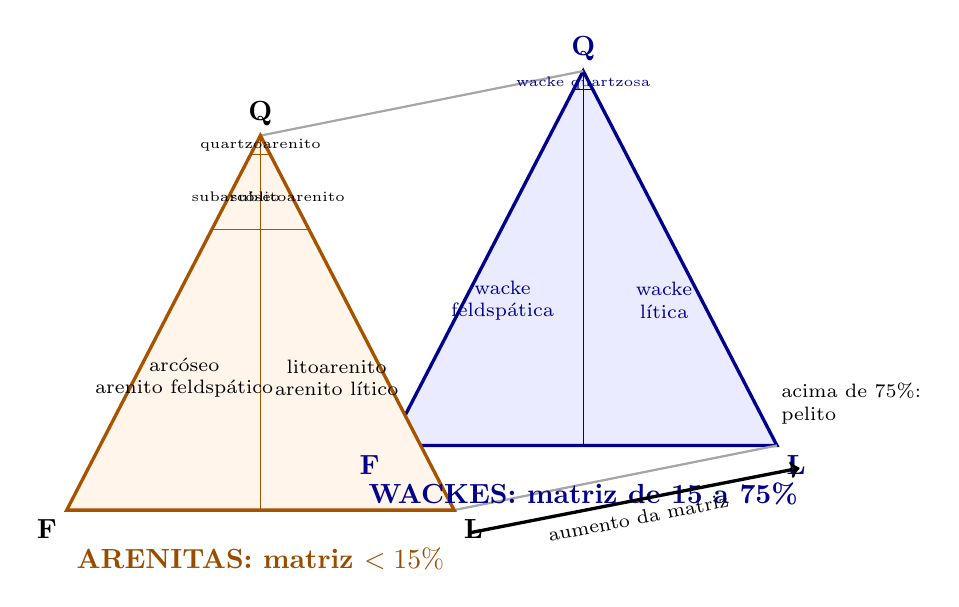
\begin{tikzpicture}[x=0.82cm,y=0.82cm,font=\scriptsize]
    % Triângulo posterior: wackes
    \coordinate (Qb) at (5,6.8);
    \coordinate (Fb) at (2,1.0);
    \coordinate (Lb) at (8,1.0);
    \path[fill=blue!8] (Qb)--(Fb)--(Lb)--cycle;
    \draw[very thick,blue!55!black] (Qb)--(Fb)--(Lb)--cycle;
    \draw[blue!55!black] (Qb)--(5,1.0);
    \draw[blue!55!black] (4.85,6.51)--(5.15,6.51);

    % Arestas que formam o prisma triangular
    \draw[gray!70,thick] (0,5.8)--(Qb);
    \draw[gray!70,thick] (-3,0)--(Fb);
    \draw[gray!70,thick] (3,0)--(Lb);

    % Triângulo anterior: arenitos/arenitas
    \coordinate (Q) at (0,5.8);
    \coordinate (F) at (-3,0);
    \coordinate (L) at (3,0);
    \path[fill=orange!8] (Q)--(F)--(L)--cycle;
    \draw[very thick,orange!65!black] (Q)--(F)--(L)--cycle;
    \draw[orange!65!black] (-0.15,5.51)--(0.15,5.51); % Q = 95%
    \draw[orange!65!black] (-0.75,4.35)--(0.75,4.35); % Q = 75%
    \draw[orange!65!black] (Q)--(0,0);                % F = L

    % Polos composicionais
    \node[above,font=\bfseries] at (Q) {Q};
    \node[below left,font=\bfseries] at (F) {F};
    \node[below right,font=\bfseries] at (L) {L};
    \node[above,font=\bfseries,text=blue!55!black] at (Qb) {Q};
    \node[below left,font=\bfseries,text=blue!55!black] at (Fb) {F};
    \node[below right,font=\bfseries,text=blue!55!black] at (Lb) {L};

    % Campos das arenitas
    \node[align=center,font=\tiny] at (0,5.65) {quartzoarenito};
    \node[align=center,font=\tiny] at (-0.38,4.85) {subarcóseo};
    \node[align=center,font=\tiny] at (0.42,4.85) {sublitoarenito};
    \node[align=center] at (-1.18,2.05) {arcóseo\\arenito feldspático};
    \node[align=center] at (1.18,2.05) {litoarenito\\arenito lítico};
    \node[font=\bfseries,orange!60!black] at (0,-0.75)
      {ARENITAS: matriz $<15\%$};

    % Campos das wackes
    \node[align=center,font=\tiny,text=blue!55!black] at (5,6.62)
      {wacke quartzosa};
    \node[align=center,text=blue!55!black] at (3.75,3.25)
      {wacke\\feldspática};
    \node[align=center,text=blue!55!black] at (6.25,3.25)
      {wacke\\lítica};
    \node[font=\bfseries,blue!55!black] at (5,0.25)
      {WACKES: matriz de 15 a 75\%};

    % Terceira dimensão do esquema
    \draw[->,very thick] (3.25,-0.35)--(8.35,0.65)
      node[midway,below,sloped] {aumento da matriz};
    \node[align=left] at (9.15,1.65) {acima de 75\%:\\pelito};
  \end{tikzpicture}